\documentclass[a4paper]{article}
\usepackage{tikz}
\usepackage{hyperref}
\usepackage{tikz}
\usetikzlibrary{patterns,arrows.meta}
\begin{document} 

\section{AULA 1}

\subsection{Lei de Coulomb}
\begin{center}
    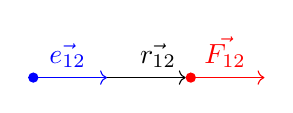
\begin{tikzpicture}
        \draw[->] (0,0) -- (2,0) node[above left] {$ \vec{r_{12}} $};
        \draw[red,Circle->](2,0) -- (3,0) node[midway,above] {$ \vec{F_{12}} $};
        \draw[blue, Circle->] (0,0) -- (1,0)node[midway,above] {$ \vec{e_{12}} $};
        \end{tikzpicture}
\end{center}

A força entre duas cargas pontuais $q_{1}$ e $q_{2}$ é dada por
\[ \vec{F}_{12} = K_e \frac{q_1 q_2}{r_{12}^2} \vec{e_{r_{12}}}\] 
onde 
\[K_e=\frac{1}{4\pi\epsilon_0} \]
\[ K_e =9*10^9 NC^{-2}m^{-2} \]
\[ \epsilon_0 = \frac{1}{4\pi*9*10^9} = 8.85*10^{-12} N^{-1}C^2m^{-2}\]
$\epsilon_0$ é conhecida como a permitividade do vácuo


\subsection{Forca Elétrica vs Força Gravítica}
\[F_g = G \frac{m_1m_2}{r^2},     F_e = K_e \frac{q_1 q_2}{r_{12}^2}\]
A força entre dois protões afastados por uma distância d
\[\frac{F_e}{F_g}= \frac{9*10^9 \frac{{(1.6*10^{-19})}^2}{d^2}}{6.7*10^{-11} \frac{{(1.7*10^{-27})}^2}{d^2}} = 10^{36}\] 
Isto é, a interação elétrica entre os dois protões é $10^{36}$
 vezes maior que a interação gravítica entre eles
,logo para partículas carregadas a interação gravítica é desprezável

\subsection{Campo Elétrico}
O campo elétrico ($\vec{E}$) é a força por unidade de carga através do 
efeito de uma carga q sobre o espaço á sua volta.
Este é dado pela divisão da lei de coulomb por $q_2$.
\[\vec{E} = \frac{\vec{F_e}}{q} = \frac{1}{4\pi\epsilon_0} \frac{Q}{r^2}\vec{e_r}\]
\[\vec{F}= q\vec{E}\]

\subsection{Principio de Sobreposição}
A força total das forças aplicadas numa carga é igual a soma vetorial 
de todas as forças que lhe são aplicadas por outras partículas
\[ \vec{E} = \sum_{i}^{}\vec{E_i} = \sum_{i}^{} \frac{1}{4\pi\epsilon_0} \frac{q_i}{r_i^2} \vec{e_{r_i}} \]

\subsection{Distribuição Contínua de Carga}
As cargas são discretas, mas num corpo carregado as suas distâncias são tão pequenas que não as conseguimos distinguir umas das outras.
É então util passar a tratar essas cargas como uma distribuição contínua

\subsubsection{Ao Longo de uma linha (1D)}
A distribuição da carga é representada por $\lambda$[C/m] medido em coulombs por metro
\[dq = \lambda dl\]

\subsubsection{Numa Superfície (2D)}
A distribuição da carga é representada por G[C/m²] medido em coulombs por metro quadrado
\[dq = Gds\]

\subsubsection{Num Volume (3D)}
A distribuição da carga é representada por $\rho$ [C/m³] medido em coulombs por metro cúbico
\[dq = \rho dv\]

\end{document}